% Chapter Template

\chapter{Theoretical Background} % Main chapter title

\label{Chapter2} % Change X to a consecutive number; for referencing this chapter elsewhere, use \ref{ChapterX}

In this section two of the most common indoor localization approaches - fingerprinting- and range-based - are reviewed. This knowledge is required to fully understand our implementation of these mechanisms. Additionally, we also include some information specific to our room recognition approach.

This chapter is organized as follows: First the range-based localization approach is introduced; the important aspects of the observation parameters (RSSI, signal propagation) and each phase of the process (ranging, weighting, trilateration) are covered in detail. Afterwards an overview over the basic fingerprint based approach is given. Finally we cover some topics specific to our room recognition approach; earth's magnetic field and support vector machine (SVM) classification.

\section{Range-Based Localization}
\label{therory:range-based}

A range based localization system consists of two main components \citep{surveyIndoorTechniques}:

\textbf{Several Anchor Nodes (ANs)}, which are placed at known locations and constantly transmit a radio signal.

\textbf{A mobile node (MN)}, in this case a smartphone, whose location is unknown and needs to be determined.

\begin{figure}[ht]
\centering
\includegraphics[width=\textwidth]{Figures/existingAproach}
\decoRule
\caption[Range-based localization approach]{Block diagram of the range based localization approach.}
\label{fig:existingApproach}
\end{figure}

To determine its position the mobile node measures the received signal strength from each of the anchor nodes $(RSSI_i)$. A ranging model is then used to estimate the distance $(d_i)$ from the mobile node to each anchor node. Because the location of the anchor nodes is known, it is then possible to calculate the position of the mobile node using trilateration. To account for errors during the ranging step the trilateration can also be provided with a set of weights $(w_i)$ representing the accuracy of each distance estimation.

The benefit of this approach is that it is not labor intensive. Compared to other approaches only a small number of training samples are required. The disadvantage is that the achievable accuracy is limited. Because of the signal propagation effects in indoor environments the ranging models are often inaccurate.

In the following subsections the ranging, trilateration and weighting steps are described in further detail.

\subsection{RSSI and signal propagation}

The received signal strength indicator describes the signal power level received by the receive radio. The measurement is given in arbitrary discrete units with higher numbers relating to a stronger signal \citep{RSSIwikipedia}.

In an open space without any obstacles the RSSI mainly depends on the propagation distance, but indoors several other factors become important. These are non line of sight (NLOS) and multi-path propagation.

NLOS occurs when the signals path is obstructed by physical objects. The signal must pass through these objects and therefore the RSSI is lower compared to LOS, where there are no obstacles \cite{JoseMaster}.

Multi-path propagation is caused when the signal is reflected from physical objects and arrives at the receiver multiple times with different signal strength. This causes inaccuracy and fluctuations in the measured RSSI as all these signals are blended together \cite{multipathEffects}.

Both effects are very common in indoor environments, caused by the walls, people, furniture and other building materials. Furthermore, the RSSI values are discrete and not fine grained what causes additional inaccuracy. This makes range-based localization based on RSSI challenging and limits its accuracy.

There are other ways to assess the signal strength, such as channel state information, which is more fine-grained and can mitigate multi-path effects, but they are not available on most mobile devices \cite{JoseMaster,FineGrainedIndoorTracking}.

\subsection{Radio-based ranging process}
\label{Ranging}

The ranging process estimates the distance between the ANs and the MN based on the radio parameters, in this case RSSI. There are several different models that can be used for ranging. In this work we use a non-linear regression (NLR) model proposed by \cite{li2015passiveWIFIsource}:
\begin{equation} \label{eqn:non-linear path loss model}
d_{i}=\alpha_{i}e^{\beta_{i}RSSI_{i}}
\end{equation}
It describes the loss of signal strength over the propagation distance. \(d_{i}\) is the estimated distance from the MN to the \(i\)-th AN, \(RSSI_{i}\) is the \(i\)-th AN's signal strength as measured by the MN and \(\alpha_{i}, \beta_{i}\) are environment variables specific to each AN.

The model needs to be trained for each AN individually by determining the values for \(\alpha_{i}\) and \(\beta_{i}\). This is done by fitting the function to a small set of training samples. This can be done using, for example, least squares optimization.

\subsection{Trilateration}

Trilateration is the process of determining an absolute or relative location based on the distance to known locations. In contrast to triangulation it relies on distances instead of angles.

In the context of localization the goal is to determine the NM's location \(\left ( x,y \right )\) based on the locations of the ANs \(\left ( \tilde{x_{i}},\tilde{y_{i}} \right )\) and the distance estimations \(d_{i}\) obtained from the path loss model.

The actual distance \(D_{i}\) from the MN to the \(i\)-th AN can be expressed as follows:
\begin{equation}
D_{i} = \sqrt{\left ( \tilde{x_{i}}-x \right )^{2}+\left ( \tilde{y_{i}}-y \right )^{2}}
\label{eqn: distance MN to AN_{i}}
\end{equation}
Under the assumption that \(d_{i}=D_{i}\) this leads to the following equation system:
\begin{equation}
\begin{pmatrix}
d_{1}\\
d_{2}\\
\vdots\\
d_{n}
\end{pmatrix}
=
\begin{pmatrix}
\sqrt{\left ( \tilde{x_{1}}-x \right )^{2}+\left ( \tilde{y_{1}}-y \right )^{2}}\\
\sqrt{\left ( \tilde{x_{2}}-x \right )^{2}+\left ( \tilde{y_{2}}-y \right )^{2}} \\
\vdots\\
\sqrt{\left ( \tilde{x_{n}}-x \right )^{2}+\left ( \tilde{y_{n}}-y \right )^{2}}
\end{pmatrix}
\label{eqn: trilateration problem as equation system}
\end{equation}

But \(d_{i}\) is only an estimation so there is no exact solution of the above system. The best solution is the one that minimizes the sum of the squared error \(d_{i} - D_{i}\). So to determine the MN's location the following problem has to be solved:
\begin{equation}
argmin_{x,y}\sum_{i=1}^{n}w_{i}\left ( d_{i} - \sqrt{\left ( \tilde{x_{i}}-x \right )^{2}+\left ( \tilde{y_{i}}-y \right )^{2}} \right )^{2}
\label{eqn: trilateration as optimization problem}
\end{equation}
To solve non-linear least squares problems the \emph{Levenberg–Marquardt} and \emph{Gauss-Newton} algorithm can be used \cite{GaussNewtonwikipedia,LevenbergMarquardtwikipedia}.

\subsection{Range weighting process}

The optimization problem in equation \ref{eqn: trilateration as optimization problem} also defines a set of weights $w_i$ corresponding to each distance estimation $d_i$. In the context of trilateration these weights represent how accurate each distance estimation is.

The ranging model's accuracy can vary greatly. By applying a large weight to the more accurate estimations and a small weight to the inaccurate ones it should, in theory, be possible to correct for the ranging error and improve the localization.

In practice the problem is that the ranging error is not known. A weighting method is needed that estimates the ranging error.

Previous work at the CDS group \cite{FineGrainedIndoorTracking} used the assumption that the ranging error is larger with increasing distance to the anchor node. So the weights were defined as inversely proportional to the estimated distances:

\begin{equation}
w_{i}=\frac{{d_i}^{-1}}{\sum_{n=1}^{N}{d_n}^{-1}}
\label{eqn: distance weights}
\end{equation}

In the remainder of this work this weighting method will be referred to as \emph{Distance Weights}.

\section{Fingerprinting-based localization}

Fingerprinting is a common method for localization based on RSSI \cite{chapre2013RSSI}. It consists of two main phases:

During the \textbf{offline/training phase}, a survey of the area of interest is performed. A map of reference points (RP) is created. Each reference point represents a known location and contains the RSSI for each AN.

Then during the \textbf{online phase}, a location positioning technique uses the currently observed signal strengths and previously collected information to figure out an estimated location. The positioning technique can employ different machine learning schemes such as k-nearest neighbor regression or support vector machines \cite{JoseMaster,surveyIndoorTechniques}.

The accuracy of this method mainly depends on the density of the RP-map. A higher density usually results in a better accuracy. Generally achieving a satisfying level of accuracy requires a lot of RPs. Other factors are the number of attributes in each RP and the variability of the observation parameters \cite{Li2012feasableMagnetic}.

More attributes per RP, an attribute being a data value like a RSSI or a magnetic field measurement, gives the algorithm more information to work with and so increased the accuracy\cite{Li2012feasableMagnetic}. This effect is subject to diminishing returns\cite{brouwers2014incremental}. A high variability in the observation parameters depending on location is also beneficial.

This approach is able to achieve good accuracies in indoor environments. The problem is that it is very labor intensive to create the necessary fingerprinting maps.

\section{Earth's magnetic field in indoor environments}

Earth's magnetic field is the magnetic field that extends from the Earth's interior out into space. It is similar to a magnetic dipole with field-lines pointing towards the magnetic north \citep{EarthMagnetwikipedia}. This feature has already been used for outdoor localization, mainly as a compass to determine the devices heading in PDR systems.

However, in indoor environments earth's magnetic field is disrupted. The presence of metal structures in the building materials, electrical devices, cables and tubes cause anomalies in the magnetic field. These anomalies make accurate heading determination difficult \citep{afzal2010assessment}.

But previous research suggests that they can be used in a fingerprinting approach to determine a devices location. The idea is that the presence of a magnetic field anomaly can be linked to a specific location. The research shows that the magnetic field anomalies are mostly stable over time and have sufficient local variability. Therefore, they should be applicable for use in localization \cite{haverinen2009global,angermann2012CharacterizationMagnetic,Li2012feasableMagnetic}.

\section{Support Vector Machine}
\label{theory:SVM}
The Support Vector Machine (SVM) is one of the most widely used machine learning algorithms. It predicts the labels of new (unknown) samples based on previous (known) examples. In its basic form it only supports two labels. This is called binary classification.

The known examples are called training data. It consists of instance-label pairs \(\left ( x_{i}, y_{i} \right ), i=1,...,l\) where \(x_{i}\in R^{n}\) and \(y_{i}\in \left \{ -1,1 \right \}\). \(x_{i}\) represents the sample's observable features while the label \(y_{i}\) defines in which category it belongs.

The SVM maps the samples into \(n\)-dimensional space. It then tries to fit a hyperplane through that space separating the two classes. Ideally all samples with \(y_{i}=1\) are on one side of the hyperplane and \(y_{i}=-1\) on the other. To make the separation as clear as possible the margin between the hyperplane and the samples is maximized at the same time. The samples that lie directly on the margins are called the support vectors.

To classify a new unknown sample the SVM determines on which side of the hyperplane it lies and assigns the according label.

To fit the hyperplane the SVM solves the following optimization problem \cite{chang2011libsvm}:
\begin{equation}
\begin{split}
\min_{\omega , b ,\xi}\;\; & \frac{1}{2}\omega^{T}\omega +C\sum_{i=1}^{l}\xi_{i}\\
\textup{subject to}\;\; & y_{i}\left ( \omega^{T}\phi \left ( x_{i} \right )+b \right )\geq 1-\xi_{i},\\
& \xi_{i}\geq 0,i=1,...,l
\end{split}
\end{equation}

There may be outliers or noise in the data. This means that a hyperplane that separates all samples correctly may not be the best classifier. To account for this a cost is paid if a sample violates the error term \(y_{i}\left ( w^{T}\phi \left ( x_{i} \right )+b \right )\geq 1\), increasing the objective function by \(C \xi_{i}\). The $C$ parameter defines the trade-off between the simplicity of the decision surface (\emph{hyperplane}) and misclassification of training samples. For large values of $C$ the optimization will chose a hyperplane with a smaller margin and more support vectors. Therefore the \emph{hyperplane} will be more complex, as it tries to classify all samples correctly. Conversely, a small value of $C$ will cause the optimizer to look for a larger-margin separating hyperplane, even if that hyperplane misclassifies some samples \cite{crossValidatedSVMC}.

\begin{figure}[htp]

\label{fig:SVM}

%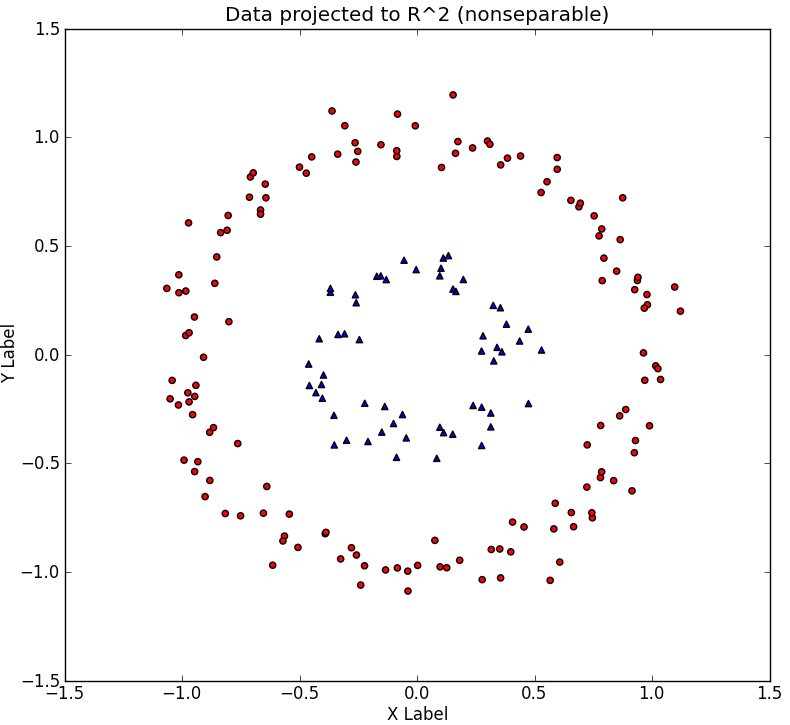
\includegraphics[width=.3\textwidth]{Figures/svm_1.png}\hfill
%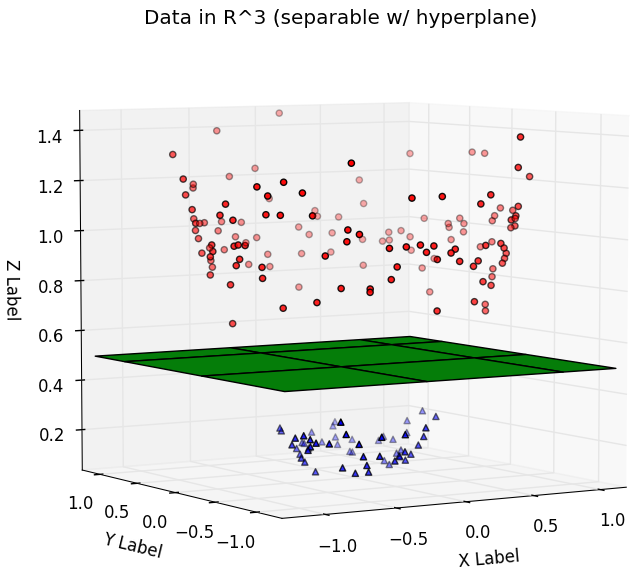
\includegraphics[width=.3\textwidth]{Figures/svm_2.png}\hfill
%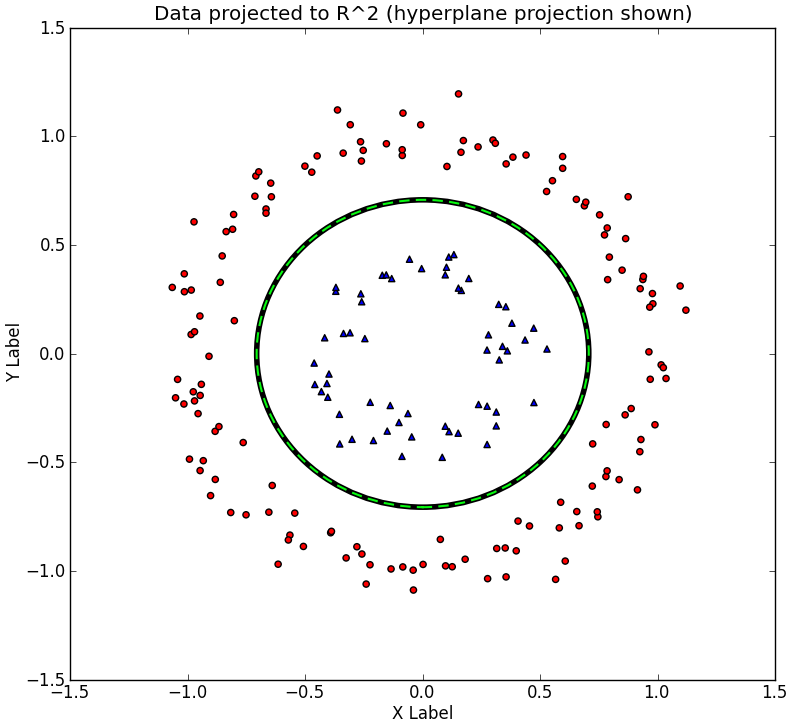
\includegraphics[width=.3\textwidth]{Figures/svm_3.png}
\centering
%\makebox[\textwidth][c]{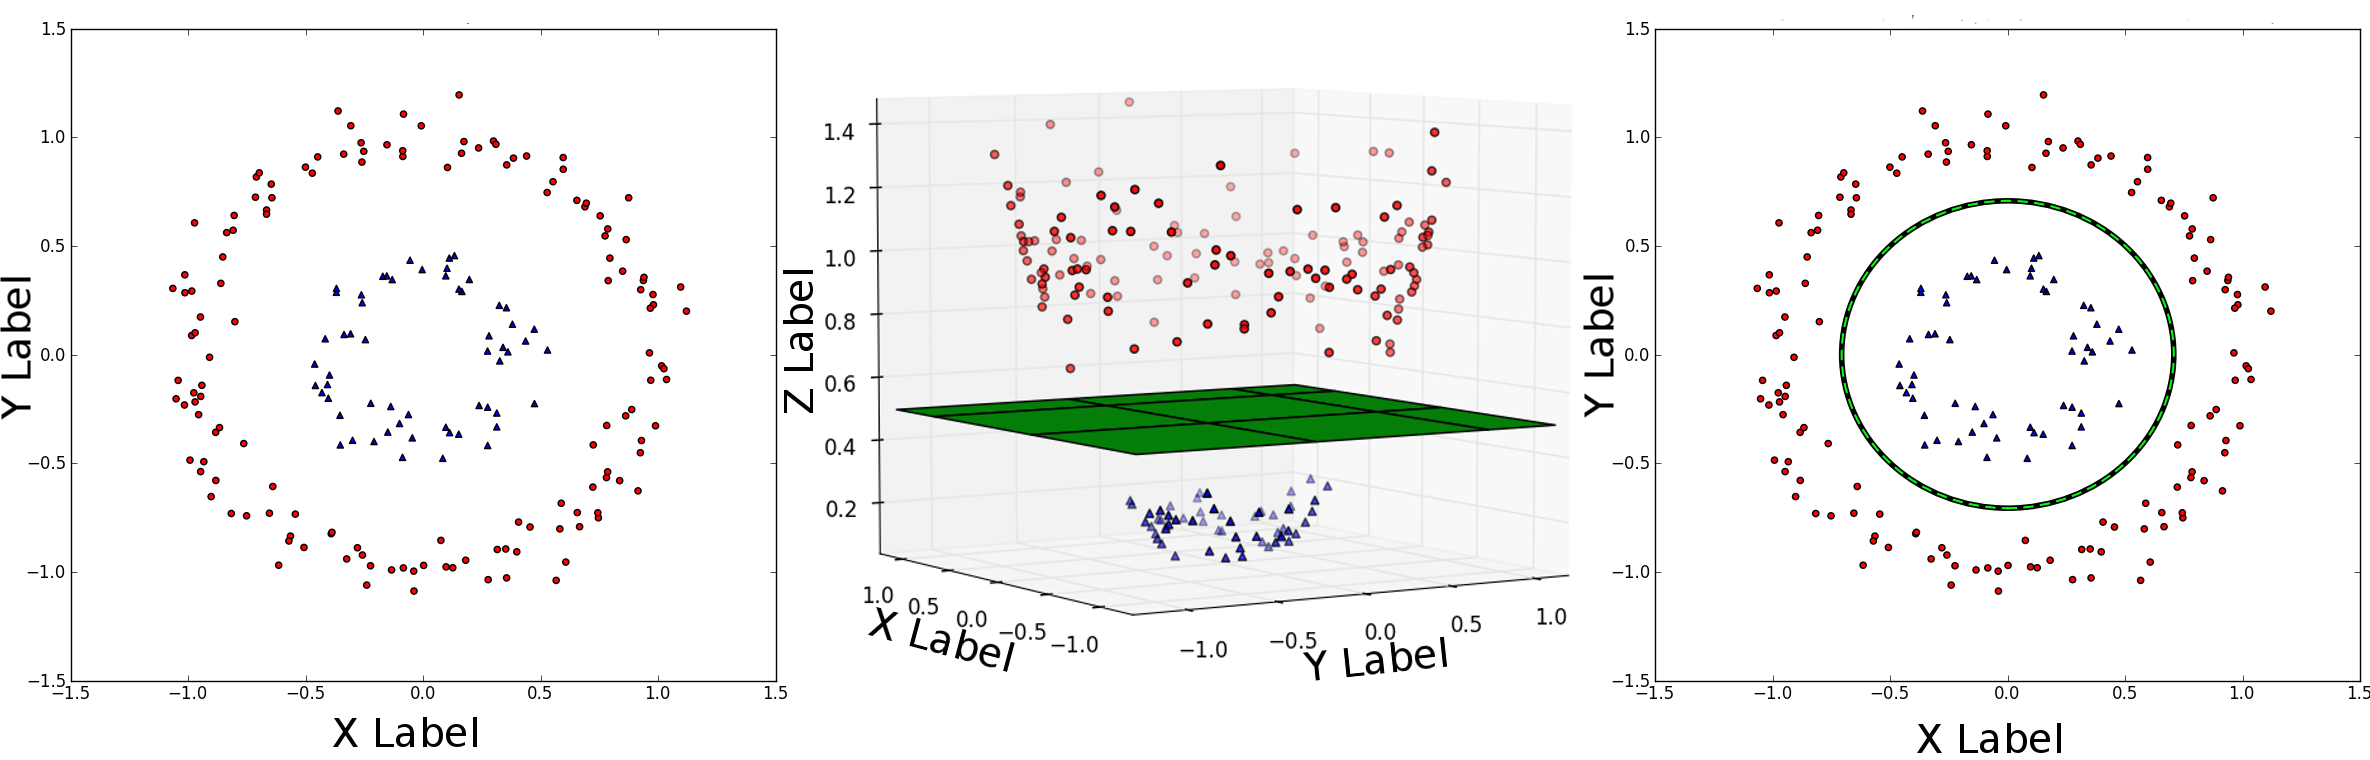
\includegraphics[width=1.3\textwidth]{Figures/svm.png}}
%\includegraphics[width=1.2\textwidth]{Figures/svm_.png}
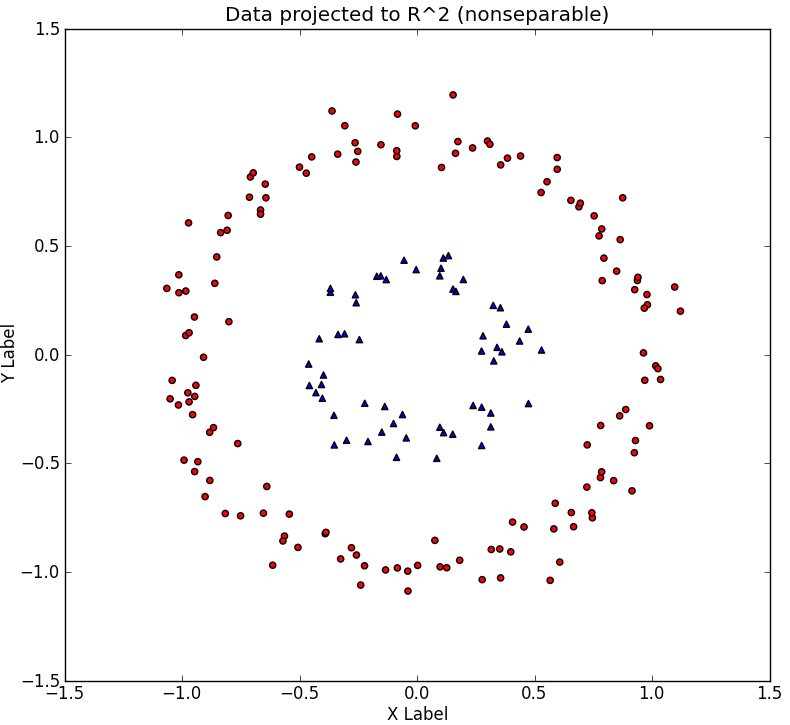
\includegraphics[width=.65\textwidth]{Figures/svm_1.png}
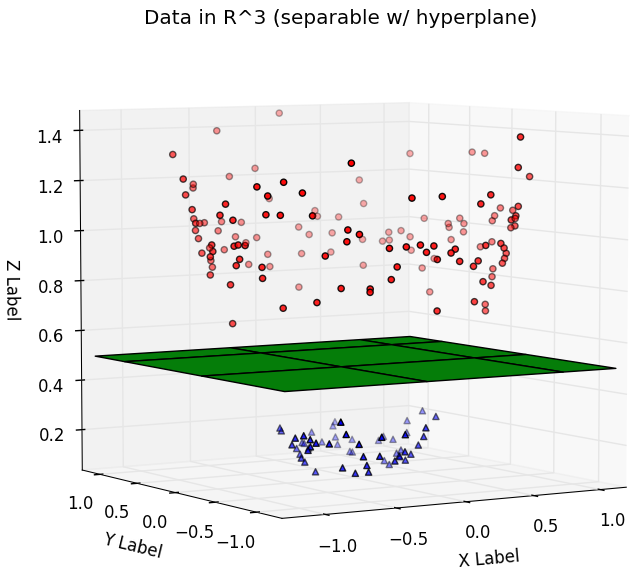
\includegraphics[width=.65\textwidth]{Figures/svm_2.png}
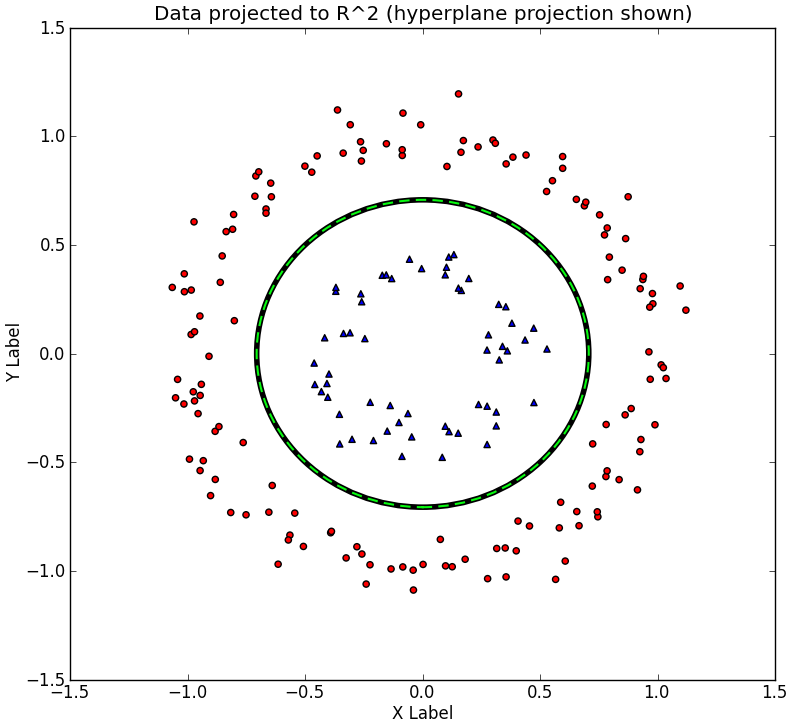
\includegraphics[width=.65\textwidth]{Figures/svm_3.png}
\decoRule
\caption[SVM kernel trick]{\raggedright(Top) A dataset in feature space, not linearly separable. (Middle)The same dataset transformed with decision boundary. (Bottom) The nonlinear decision boundary.}

\end{figure}

But the training data may not be linearly separable. In this case the so-called kernel trick can be used. The kernel is a function \(k\left ( x_{i}, x_{j} \right )=\phi \left ( x_{i} \right )\cdot \phi\left ( x_{j} \right )\), which maps the features \(x_{i}\) to a higher dimensional space where they can be separated by a hyperplane. This results in a non-linear separation in the original feature space \cite{ErikKimKernelTrick}.

To perform multi-class classification the "one-against-one" approach can be used. For \(k\) classes \(k\left ( k-1 \right )/2\) classifiers are trained. Each binary classifier is then considered to vote for a class. The sample is then placed in the class with the most votes \cite{chang2011libsvm}.
